\section{Unsteady Groundwater Flow}
\subsection{Confined Aquifers}
\subsubsection{Finite-Difference Methods -- 1 Spatial Dimension}
Using Equation \ref{eqn:confined-aquifer-flow-PDE} as a starting point for simulating aquifer behavior, the unsteady flow condition means that the left hand side remains.
 \begin{equation}
S \Delta x \Delta y  \frac{h_{i}^{t+\Delta t} - h_{i}^{t}}{\Delta t} = 
(K \Delta y \Delta z \frac{h_{i-1} - h_{i}}{\Delta x}) - 
(K \Delta y \Delta z \frac{h_{i} - h_{i+1}}{\Delta x})
\end{equation}

Next we will use the arithmetic mean values of the material properties ($K$) at the cell interfaces, so the difference equation becomes
 \begin{equation}
S \Delta x \Delta y  \frac{h_{i}^{t+\Delta t} - h_{i}^{t}}{\Delta t} = 
(\frac{1}{2}(K_{i-1}+K_{i}) \Delta y \Delta z \frac{h_{i-1} - h_{i}}{\Delta x}) - 
(\frac{1}{2}(K_{i}+K_{i-1}) \Delta y \Delta z \frac{h_{i} - h_{i+1}}{\Delta x})
\end{equation}

Now divide both sides by $\Delta x \Delta y$ to obtain
 \begin{equation}
S  \frac{h_{i}^{t+\Delta t} - h_{i}^{t}}{\Delta t} = 
(\frac{1}{2}(K_{i-1}+K_{i})  \Delta z \frac{h_{i-1} - h_{i}}{\Delta x^2}) - 
(\frac{1}{2}(K_{i}+K_{i-1})  \Delta z \frac{h_{i} - h_{i+1}}{\Delta x^2})
\end{equation}

Multiply by $\frac{\Delta t}{S_{i}}$ to obtain
 \begin{equation}
  h_{i}^{t+\Delta t} - h_{i}^{t} = 
\frac{\Delta t}{S_{i}} \times [ (\frac{1}{2}(K_{i-1}+K_{i})  \Delta z \frac{h_{i-1} - h_{i}}{\Delta x^2}) - 
(\frac{1}{2}(K_{i}+K_{i-1})  \Delta z \frac{h_{i} - h_{i+1}}{\Delta x^2}) ]
\end{equation}

Now lets group some constants:
\begin{equation}
\begin{matrix}
A_{i} = \frac{\Delta t}{2 S_i \Delta x^2}(K_{i-1}+K_{i}) \Delta z \\
~ \\
B_{i} = \frac{\Delta t}{2 S_i \Delta x^2}(K_{i}+K_{i+1}) \Delta z
\end{matrix}
\end{equation}

Now substitute into the difference equation.

\begin{equation}
h_{i}^{t + \Delta t} = A_{i}(h_{i-1}^{*}) -(A_{i}+B_{i})(h_{i})^{*}+ B_{i}(h_{i+1}^{*}) + h_{i}^t
\end{equation}

Next we have to decide what time level to evaluate the right hand side terms that have the $^{*}$ time superscript.
\subsubsection{Explicit Formulation}
If we choose to evaluate at the current time step, the method is called an explicit method.  
It works fine, but stability requirements force us to use ratios of space and time steps that are often limiting --- this behavior is called ``conditional stability.'' 
\begin{equation}
h_{i}^{t + \Delta t} = A_{i}(h_{i-1}^{t}) -(A_{i}+B_{i})(h_{i})^{t}+ B_{i}(h_{i+1}^{t}) + h_{i}^t
\end{equation}
The advantage of this construct is simplicity for programming -- in fact one can actually solve these kind of problem graphically if you choose a proper space and time step.

\subsubsection{Implicit Formulation}
If instead we choose to evaluate at the new time step, the method is called an implicit method. 
\begin{equation}
h_{i}^{t + \Delta t} = A_{i}(h_{i-1}^{t + \Delta t}) -(A_{i}+B_{i})(h_{i}^{t + \Delta t})+ B_{i}(h_{i+1}^{t + \Delta t}) + h_{i}^t
\end{equation}
A slight rearrangement of the equation produces a structure very amenable to Jacobi iteration (with all its faults!)
\begin{equation}
0= A_{i}(h_{i-1}^{t + \Delta t}) -(A_{i}+B_{i}+1)(h_{i}^{t + \Delta t})+ B_{i}(h_{i+1}^{t + \Delta t}) + h_{i}^t
\end{equation}
If indeed we decide to use Jacobi iteration, then the system to be solved is
\begin{equation}
h_{i}^{t + \Delta t} = \frac{A_{i}(h_{i-1}^{t + \Delta t}) + B_{i}(h_{i+1}^{t + \Delta t}) + h_{i}^t}{A_{i}+B_{i}+1}
\end{equation}

\subsection{Finite-Difference Methods -- 2 Spatial Dimensions}
Rather than build a 1D example, in this section we will just build a 2D example.  
We will use a fully-implicit method to take advantage of our Jacobi solver we have already built, and incorporate both the boundary condtion masks and a pumping array. 
The result will be a functional tool, that with some further modifications could be used for actual groundwater engineering problems, albeit the computations would seem quite slow. 
However, a few hours of run time is a lot loss costly than drilling wells in the wrong places --- for a professional problem we would probably use MODFLOW which has far more efficient solvers (but interestingly works about the same).\footnote{At the conclusion of the example, we will compare the results to MODFLOW and demonstrate that the two tools produce the same answers.  Generally we won't often have to build our own codes -- however if we do, they should produce the same results as a professional code for the same problem.  Then we would use our homebuilt code for whatever special need we have that the professional code cannot conveniently address.}

Starting with
\begin{equation}
\begin{matrix}
S \frac{\partial h_i}{\partial t} = 
[\frac{1}{\Delta x} T_{x} \frac{h_{i-1,j} - h_{i,j}}{\Delta x} +
 \frac{1}{\Delta y} T_{y} \frac{h_{i,j-1} - h_{i,j}}{\Delta y}] - \\
~~~~~~~~~~\\
~~~~~~~~~~[ \frac{1}{\Delta x} T_{x}  \frac{h_{i,j} - h_{i+1,j}}{\Delta x} +
  \frac{1}{\Delta y}  T_{y} \frac{h_{i,j} - h_{i,j+1}}{\Delta y} ]  \\
  ~~~~~~~\\
  + \frac{R_{i,j}}{\Delta x \Delta y} - \frac{Q_{i,j}}{\Delta x \Delta y} \\     
\end{matrix}        
\end{equation}

We apply the finite difference approach to the time derivative and obtain

\begin{equation}
\begin{matrix}
S \frac{h_i^{t+\Delta t}-h_i^{t}}{\Delta t} = 
[\frac{1}{\Delta x} T_{x} \frac{h_{i-1,j} - h_{i,j}}{\Delta x} +
 \frac{1}{\Delta y} T_{y} \frac{h_{i,j-1} - h_{i,j}}{\Delta y}] - \\
~~~~~~~~~~\\
~~~~~~~~~~[ \frac{1}{\Delta x} T_{x}  \frac{h_{i,j} - h_{i+1,j}}{\Delta x} +
  \frac{1}{\Delta y}  T_{y} \frac{h_{i,j} - h_{i,j+1}}{\Delta y} ]  \\
  ~~~~~~~\\
  + \frac{R_{i,j}}{\Delta x \Delta y} - \frac{Q_{i,j}}{\Delta x \Delta y} \\     
\end{matrix}        
\end{equation}

Proceeding as above in the 1D case, we will isolate the time levels, multiply through by $\Delta t$, and divide by $S$ we obtain

\begin{equation}
\begin{matrix}
h_i^{t+\Delta t} = h_i^{t} +
\frac{~\Delta t}{S_i}~[\frac{1}{\Delta x} T_{x} \frac{h_{i-1,j} - h_{i,j}}{\Delta x} +
 \frac{1}{\Delta y} T_{y} \frac{h_{i,j-1} - h_{i,j}}{\Delta y}] - \\
~~~~~~~~~~\\
~~~~~~~~~~\frac{~\Delta t}{S_i}~[ \frac{1}{\Delta x} T_{x}  \frac{h_{i,j} - h_{i+1,j}}{\Delta x} +
  \frac{1}{\Delta y}  T_{y} \frac{h_{i,j} - h_{i,j+1}}{\Delta y} ]  \\
  ~~~~~~~\\
  +\frac{~\Delta t}{S_i}~ \frac{R_{i,j}}{\Delta x \Delta y} - \frac{~\Delta t}{S_i}~\frac{Q_{i,j}}{\Delta x \Delta y} \\     
\end{matrix}        
\end{equation}

Next if we choose the time level on the right-hand side as $t$, we would have an explicit scheme\footnote{Easy to program, but conditionally stable and usually requiring a very small time step for stability.  Here we will use an implicit scheme, which will be unconditionally stable -- we will still use pretty small time steps for accuracy, but not need to worry too much about stability.}, however if we choose to evaluate at the new time level $t + \Delta t$, we have an implicit scheme.  
We are going to choose an implicit scheme to leverage our work on the Jacobi solver we have already built so the difference equation becomes

\begin{equation}
\begin{matrix}
h_i^{t+\Delta t} = h_i^{t} +
\frac{~\Delta t}{S_i}~[\frac{1}{\Delta x} T_{x} \frac{h_{i-1,j}^{t+\Delta t} - h_{i,j}^{t+\Delta t}}{\Delta x} +
 \frac{1}{\Delta y} T_{y} \frac{h_{i,j-1}^{t+\Delta t} - h_{i,j}^{t+\Delta t}}{\Delta y}] - \\
~~~~~~~~~~\\
~~~~~~~~~~\frac{~\Delta t}{S_i}~[ \frac{1}{\Delta x} T_{x}  \frac{h_{i,j}^{t+\Delta t} - h_{i+1,j}^{t+\Delta t}}{\Delta x} +
  \frac{1}{\Delta y}  T_{y} \frac{h_{i,j}^{t+\Delta t} - h_{i,j+1}^{t+\Delta t}}{\Delta y} ]  \\
  ~~~~~~~\\
  +\frac{~\Delta t}{S_i}~ \frac{R_{i,j}^{t}}{\Delta x \Delta y} - \frac{~\Delta t}{S_i}~\frac{Q_{i,j}^{t}}{\Delta x \Delta y} \\     
\end{matrix}        
\label{eqn:fdm-unsteady-confined}
\end{equation}

Equation \ref{eqn:fdm-unsteady-confined} is the difference equation we will code into our \textbf{R} script with some modifications to allow time stepping and plotting results.
I set the pumping and recharge at time level $t$, but one could just as well choose to average over two time levels.
As long as the time steps are small relative to changes in pumping and recharge\footnote{Stress periods on the order of months for time steps in days}, it won't make much practical difference.

Observe a very important part of the difference equation, $h_i^{t}$ is known at the beginning of a time step and does not change during the computation effort for that time period -- it is just another constant like recharge or pumping.   
However, once we have the update, then it is changed and the next time step is begun.
The observation is important to remember because we are simply going to wrap a time stepping loop around our already tested and working Jacobi solver.

Employing the same $A,B,C,D$ structure as the unsteady 2D solvers we built the update model is

Also as in the one-dimensional case, we will approximate the spatial variation of the material properties (transmissivity) as arithmetic mean values between two cells, so making the following definitions:

\begin{equation}
\begin{matrix}
A_{i,j} = \frac{\Delta t}{2 S_i~\Delta x^2}(T_{x,(i-1,j)}+T_{x,(i,j)}) \\ ~~ \\
B_{i,j} = \frac{\Delta t}{2 S_i~\Delta x^2}(T_{x,(i,j)}+T_{x,(i+1,j)})   \\ ~~ \\
C_{i,j} = \frac{\Delta t}{2 S_i~\Delta y^2}(T_{y,(i,j-1)}+T_{y,(i,j)})   \\ ~~ \\
D_{i,j} = \frac{\Delta t}{2 S_i~\Delta y^2}(T_{y,(i,j)}+T_{y,(i,j+1)})   \\ ~~ \\
E_{i,j} = \frac{~\Delta t}{S_i~\Delta x \Delta y}
\end{matrix}
\end{equation}

Substitution into the difference equation and writing the cell equation for $h_{i,j}$ yields

\begin{equation}
h_{i,j}^{t+\Delta t} = \frac{[A_{i,j}h_{i-1,j}^{t+\Delta t} + B_{i,j}h_{i+1,j}^{t+\Delta t} + C_{i,j}h_{i,j-1}^{t+\Delta t} + D_{i,j}h_{i,j+1}^{t+\Delta t}]}{[A_{i,j}+B_{i,j}+C_{i,j}+D_{i,j}+1]}+h_{i}^{t}+E_{i,j}[R_{i,j}^{t}-Q_{i,j}^{t}]\\
\end{equation}

This equation is quite amenable to the Jacobi iteration technique, with the addition of the two left-most terms for head at the start of the time step and the net recharge less pumping. 
Notice the $+1$ in the denominator of the weighting term -- it reflects that $h_{i,j}^{t+\Delta t}$ appears on both the left and right hand side of Equation \ref{eqn:fdm-unsteady-confined}.

Listing \ref{lst:2D-Unsteady} is an \textbf{R} script that implements these changes.
In the script the plotting has been moved into the prototype function, so we can generate a plot when we wish.
The input data reading portion has a line added to capture the time step length, the maximum number of time steps to take, a printing frequency (make a plot every \texttt{iprint} time steps), and a storage coefficient array.
Observe that the printing test makes use of the \texttt{MODULO} construct in \textbf{R}.

The actual script use will be demonstrated by the next example.

\begin{lstlisting}[caption= R code demonstrating an Aquifer Flow Simulator for 2D Unsteady Confined Aquifer Flow.  This code fragment implements the Jacobi iteration to solve the linear system at \textbf{each time step}.  A plotting prototype function is used so we can plot to a graphics device at specified intervals (multiples of the total number of time steps).  A graphics device is used (rather than plotting to the \textbf{R Studio} environment) so multiple plots at different simulation times can be rendered , label=lst:2D-Unsteady]
# 2D Unsteady Confined -- With Boundary Arrays and Wells using Jacobi Iteration
# deallocate memory
rm(list=ls())
##############################################################
# prototype plotting function                                #
##############################################################
plotnow<-function(headnow,ncols,nrows,etime,deltat){
###    built position arrays for contour plotting         
velocity_plt<-matrix(0,ncols,nrows) 
for( i in 1:nrows){
  for( j in 1:ncols){
    velocity_plt[j,i]=headnow[i,j]
  }
}
###    contour plot of head -- note axes are rotated
#debug  message("elapsed time : ",maxtime * deltat)
mytitle <- paste("Head (Blue) Map at Time = :",etime*deltat," seconds")
contour(distancex,distancey,velocity_plt,
        plot.title = title(main = mytitle,
                           xlab = "Meters (X axis) ====>>", 
                           ylab = "Meters (Y axis) ====>>"),
        col="blue",lwd=3,nlevels=20)
}
################################################################
################################################################
zz <- file("input2.dat", "r") # Open a connection named zz to file named input.dat
# read the simulation conditons
deltax <-as.numeric(readLines(zz, n = 1, ok = TRUE, warn = TRUE,encoding = "unknown", skipNul = FALSE))
deltay <-as.numeric(readLines(zz, n = 1, ok = TRUE, warn = TRUE,encoding = "unknown", skipNul = FALSE))
deltaz <-as.numeric(readLines(zz, n = 1, ok = TRUE, warn = TRUE,encoding = "unknown", skipNul = FALSE))
deltat <-as.numeric(readLines(zz, n = 1, ok = TRUE, warn = TRUE,encoding = "unknown", skipNul = FALSE))
nrows <-as.numeric(readLines(zz, n = 1, ok = TRUE, warn = TRUE,encoding = "unknown", skipNul = FALSE))
ncols <-as.numeric(readLines(zz, n = 1, ok = TRUE, warn = TRUE,encoding = "unknown", skipNul = FALSE))
tolerance <- as.numeric(readLines(zz, n = 1, ok = TRUE, warn = TRUE,encoding = "unknown", skipNul = FALSE))
maxiter <- as.numeric(readLines(zz, n = 1, ok = TRUE, warn = TRUE,encoding = "unknown", skipNul = FALSE))
maxtime <- as.numeric(readLines(zz, n = 1, ok = TRUE, warn = TRUE,encoding = "unknown", skipNul = FALSE))
iprint <- as.numeric(readLines(zz, n = 1, ok = TRUE, warn = TRUE,encoding = "unknown", skipNul = FALSE))
distancex <- (readLines(zz, n = 1, ok = TRUE, warn = TRUE,encoding = "unknown", skipNul = FALSE))
distancey <- (readLines(zz, n = 1, ok = TRUE, warn = TRUE,encoding = "unknown", skipNul = FALSE))
# add boundary conditions 0= fixed head, 1= no flow
boundarytop <- (readLines(zz, n = 1, ok = TRUE, warn = TRUE,encoding = "unknown", skipNul = FALSE))
boundarybottom <- (readLines(zz, n = 1, ok = TRUE, warn = TRUE,encoding = "unknown", skipNul = FALSE))
boundaryleft <- (readLines(zz, n = 1, ok = TRUE, warn = TRUE,encoding = "unknown", skipNul = FALSE))
boundaryright <- (readLines(zz, n = 1, ok = TRUE, warn = TRUE,encoding = "unknown", skipNul = FALSE))
hydhead <-(readLines(zz, n = nrows, ok = TRUE, warn = TRUE,encoding = "unknown", skipNul = FALSE))
# hydhead is now the initial condition array #
hydcondx <-(readLines(zz, n = nrows, ok = TRUE, warn = TRUE,encoding = "unknown", skipNul = FALSE))
hydcondy <-(readLines(zz, n = nrows, ok = TRUE, warn = TRUE,encoding = "unknown", skipNul = FALSE))
storage <-(readLines(zz, n = nrows, ok = TRUE, warn = TRUE,encoding = "unknown", skipNul = FALSE))
pumping <-(readLines(zz, n = nrows, ok = TRUE, warn = TRUE,encoding = "unknown", skipNul = FALSE)) 
close(zz)
# split the multiple column strings into numeric components for a vector
distancex <-as.numeric(unlist(strsplit(distancex,split=" ")))
distancey <-as.numeric(unlist(strsplit(distancey,split=" ")))
boundarytop <-as.numeric(unlist(strsplit(boundarytop,split=" ")))
boundarybottom <-as.numeric(unlist(strsplit(boundarybottom,split=" ")))
boundaryleft <-as.numeric(unlist(strsplit(boundaryleft,split=" ")))
boundaryright <-as.numeric(unlist(strsplit(boundaryright,split=" ")))
hydhead <-as.numeric(unlist(strsplit(hydhead,split=" ")))
hydcondx <-as.numeric(unlist(strsplit(hydcondx,split=" ")))
hydcondy <-as.numeric(unlist(strsplit(hydcondy,split=" ")))
storage <-as.numeric(unlist(strsplit(storage,split=" ")))
pumping <-as.numeric(unlist(strsplit(pumping,split=" ")))
# convert the numeric vectors into matrices for easier indexing
hydhead <- matrix(hydhead,nrow=nrows,ncol=ncols,byrow = TRUE)
hydcondx <-matrix(hydcondx,nrow=nrows,ncol=ncols,byrow = TRUE)
hydcondy <-matrix(hydcondy,nrow=nrows,ncol=ncols,byrow = TRUE)
storage <-matrix(storage,nrow=nrows,ncol=ncols,byrow = TRUE)
pumping <-matrix(pumping,nrow=nrows,ncol=ncols,byrow = TRUE)
# allocate a graphics device for sequential plotting
pdf("2d-unsteady-confined-junk.plot.pdf") # send any plots to file
# here we perform the velocity potential calculations
# built the transmissivity arrays
amat<-matrix(0,nrows,ncols) 
bmat<-matrix(0,nrows,ncols) 
cmat<-matrix(0,nrows,ncols)
dmat<-matrix(0,nrows,ncols)
qrat<-matrix(0,nrows,ncols)
for(irow in 2:(nrows-1)){
  for(jcol in 2:(ncols-1)){
    amat[irow,jcol]<-((hydcondx[irow-1,jcol  ]+hydcondx[irow  ,jcol  ])*deltat*deltaz)/(2.0*storage[irow,jcol]*deltax^2)
    bmat[irow,jcol]<-((hydcondx[irow  ,jcol  ]+hydcondx[irow+1,jcol  ])*deltat*deltaz)/(2.0*storage[irow,jcol]*deltax^2)
    cmat[irow,jcol]<-((hydcondy[irow  ,jcol-1]+hydcondy[irow  ,jcol  ])*deltat*deltaz)/(2.0*storage[irow,jcol]*deltay^2)
    dmat[irow,jcol]<-((hydcondy[irow  ,jcol  ]+hydcondy[irow  ,jcol+1])*deltat*deltaz)/(2.0*storage[irow,jcol]*deltay^2)
    qrat[irow,jcol]<-(-1.0)*deltat*pumping[irow,jcol]/(deltax*deltay*storage[irow,jcol])
    }
}
####### initial conditions ######################################
headnow <- hydhead
for (tstep in 1:maxtime){   ### this is the outer time-stepping loop
###### use jacobi to solve for a single time step ###############
hydhead <- headnow
headold <- hydhead # copy the head array, used to test for stopping
tolflag <- FALSE
for (iter in 1:maxiter){
# Boundary Conditions
# Top Row
for(jcol in 1:ncols){
    if(boundarytop[jcol] == 0){hydhead[1,jcol]<-hydhead[2,jcol]} #no-flow at top
    if(boundarybottom[jcol] == 0){hydhead[nrows,jcol]<-hydhead[2,jcol]} #no-flow at bottom
    # otherwise values are fixed head
}
for(irow in 1:nrows){
    if(boundaryleft[irow] == 0){hydhead[irow,1]<-hydhead[irow,2]} #no-flow at left
    if(boundaryright[irow] == 0){hydhead[irow,ncols]<-hydhead[irow,ncols-1]} #no-flow at right
}
  for (irow in 2:(nrows-1)){
    for (jcol in 2:(ncols-1)){
      hydhead[irow,jcol] <- (  headnow[irow,jcol] +
                                  qrat[irow,jcol] +
           amat[irow,jcol]*hydhead[irow-1,jcol  ] +
           bmat[irow,jcol]*hydhead[irow+1,jcol  ] +
           cmat[irow,jcol]*hydhead[irow  ,jcol-1] +
           dmat[irow,jcol]*hydhead[irow  ,jcol+1] )/
        (amat[irow,jcol]+bmat[irow,jcol]+cmat[irow,jcol]+dmat[irow,jcol]+1)
    }
  }
  # test for stopping iterations
  percentdiff <- sum((hydhead-headold)^2)
  if (percentdiff < tolerance){
    message("Exit iterations in velocity potential because tolerance met");
    message("Iterations =", iter);
    message("Current error : ",percentdiff);
    tolflag <- TRUE
    break
  }
 headold<-hydhead  #update the current head vector
# if( iter %% 1000 == 0){message("Calculating in Potential Function ",iter," of ",maxiter, " iterations")}
}
if (tolflag == FALSE){
#  message("Exit iterations in potential function at max iterations")
  message("Current error : ",percentdiff)
  }
# perform an update
headnow <- hydhead
########## end of a time step ################################
# check for plotnow
if(tstep%%iprint==0){plotnow(headnow,ncols,nrows,tstep,deltat)}
}
# exit the time-stepping loop
# output ending conditons
write(t(hydhead), file='2d-unsteady-confined.txt',ncolumns = ncols,sep=",")
# deallocate (disconnect) graphics device
dev.off() # disconect the pdf file
\end{lstlisting}

\textbf{Example 1: Rectangular Aquifer with Pumping -- Unsteady Flow}
Figure \ref{fig:Hubbleville} is a plan view of a confined aquifer with a Well field located as shown, near the Red River.
The head in the river is 1000 meters as is the head at the South boundary, the Green Swamp.
The aquifer thickness is about 10 meters.
The hydraulic conductivity of the water producing zone is 20 meters per day.
Determine the head distribution every 100 days of pumping at a rate of 20,000 cubic meters per day for 1000 days (about 3 years).
The storage coefficient of the aquifer is $S=0.01$.
\begin{figure}[h!] %  figure placement: here, top, bottom, or page
   \centering
   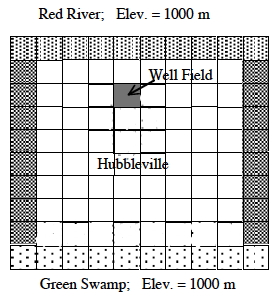
\includegraphics[height=4in]{./18-UnsteadyGroundwaterFlow/Hubbleville.jpg} 
   \caption{Rectangular aquifer with wellfield.  North and South boundaries are fixed head.  East and West boundaries are Zero-Flux}
   \label{fig:Hubbleville}
\end{figure}

Each cell in the sketch is $1000 X 1000$ meters.

Listing \ref{lst:HubblevilleInput} is the input file for the example problem.  
Literally it only has two new ``lines.''

\begin{lstlisting}[caption= Input file for the Hubbleville Aquifer Example.  Annotations in the listing need to be removed for actual running of the file and are included to illustrate the various parts of the input data , label=lst:HubblevilleInput]
1000 <== Delta x
1000 <== Delta y
10 <== Delta z (thickness)
0.1 <== Time step length (in days)
10 <==row count
10 <== column count
1e-8 <== tolerance for linear solver
1000 <== how many trials per linear system
10000 <== how many time steps
1000 <== print every ## time step
0 1000 2000 3000 4000 5000 6000 7000 8000 9000 
0 1000 2000 3000 4000 5000 6000 7000 8000 9000
1 1 1 1 1 1 1 1 1 1   <== boundary conditions
1 1 1 1 1 1 1 1 1 1
0 0 0 0 0 0 0 0 0 0
0 0 0 0 0 0 0 0 0 0
1000 1000 1000 1000 1000 1000 1000 1000 1000 1000  <== initial head array 
1000 1000 1000 1000 1000 1000 1000 1000 1000 1000 
1000 1000 1000 1000 1000 1000 1000 1000 1000 1000 
1000 1000 1000 1000 1000 1000 1000 1000 1000 1000 
1000 1000 1000 1000 1000 1000 1000 1000 1000 1000 
1000 1000 1000 1000 1000 1000 1000 1000 1000 1000 
1000 1000 1000 1000 1000 1000 1000 1000 1000 1000 
1000 1000 1000 1000 1000 1000 1000 1000 1000 1000 
1000 1000 1000 1000 1000 1000 1000 1000 1000 1000 
1000 1000 1000 1000 1000 1000 1000 1000 1000 1000 
20 20 20 20 20 20 20 20 20 20 20 20  <== Kx array
20 20 20 20 20 20 20 20 20 20 20 20
20 20 20 20 20 20 20 20 20 20 20 20
20 20 20 20 20 20 20 20 20 20 20 20
20 20 20 20 20 20 20 20 20 20 20 20
20 20 20 20 20 20 20 20 20 20 20 20
20 20 20 20 20 20 20 20 20 20 20 20
20 20 20 20 20 20 20 20 20 20 20 20
20 20 20 20 20 20 20 20 20 20 20 20
20 20 20 20 20 20 20 20 20 20 20 20
20 20 20 20 20 20 20 20 20 20 20 20  <== Ky array
20 20 20 20 20 20 20 20 20 20 20 20
20 20 20 20 20 20 20 20 20 20 20 20
20 20 20 20 20 20 20 20 20 20 20 20
20 20 20 20 20 20 20 20 20 20 20 20
20 20 20 20 20 20 20 20 20 20 20 20
20 20 20 20 20 20 20 20 20 20 20 20
20 20 20 20 20 20 20 20 20 20 20 20
20 20 20 20 20 20 20 20 20 20 20 20
20 20 20 20 20 20 20 20 20 20 20 20
0.01 0.01 0.01 0.01 0.01 0.01 0.01 0.01 0.01 0.01 <== Storage coefficient
0.01 0.01 0.01 0.01 0.01 0.01 0.01 0.01 0.01 0.01
0.01 0.01 0.01 0.01 0.01 0.01 0.01 0.01 0.01 0.01
0.01 0.01 0.01 0.01 0.01 0.01 0.01 0.01 0.01 0.01
0.01 0.01 0.01 0.01 0.01 0.01 0.01 0.01 0.01 0.01
0.01 0.01 0.01 0.01 0.01 0.01 0.01 0.01 0.01 0.01
0.01 0.01 0.01 0.01 0.01 0.01 0.01 0.01 0.01 0.01
0.01 0.01 0.01 0.01 0.01 0.01 0.01 0.01 0.01 0.01
0.01 0.01 0.01 0.01 0.01 0.01 0.01 0.01 0.01 0.01
0.01 0.01 0.01 0.01 0.01 0.01 0.01 0.01 0.01 0.11
0 0 0 0 0 0 0 0 0 0 <== pumping array
0 0 0 0 0 0 0 0 0 0
0 0 0 0 0 0 0 0 0 0
0 0 0 0 0 0 0 0 0 0
0 0 0 0 0 0 0 0 0 0
0 0 0 0 0 0 0 0 0 0
0 0 0 0 0 0 0 0 0 0
0 0 0 0 20000 0 0 0 0 0
0 0 0 0 0 0 0 0 0 0
0 0 0 0 0 0 0 0 0 0
\end{lstlisting}

Figures \ref{fig:HubblevillePlot300} and \ref{fig:HubblevillePlot900} are plots of the head distribution after 300 and 900 days (in the first year and the third year of pumping).
In the plots one can observe that the cone of depression is growing (outward from the well field), and the numerical values of the contours are reflecting the progressively declining head elevations.

At some point the head distribution would stop changing (and equilibrium solution) and would agree with a steady flow simulation for the same aquifer conditions.
If one were to perform a ``cut-and-fill'' analysis of the contour maps, the amount of aquifer dewatered (difference in head multiplied by the storage coefficient, integrated over the entire area shown) would equal the volume pumped from the system.\footnote{Numerically very close -- there might be some differences because of arithmetic precision issues.}

The next section will extend the concept to an unconfied aquifer -- again using the variable transmissivity approach of the prior chapter.

\begin{figure}[h!] %  figure placement: here, top, bottom, or page
   \centering
   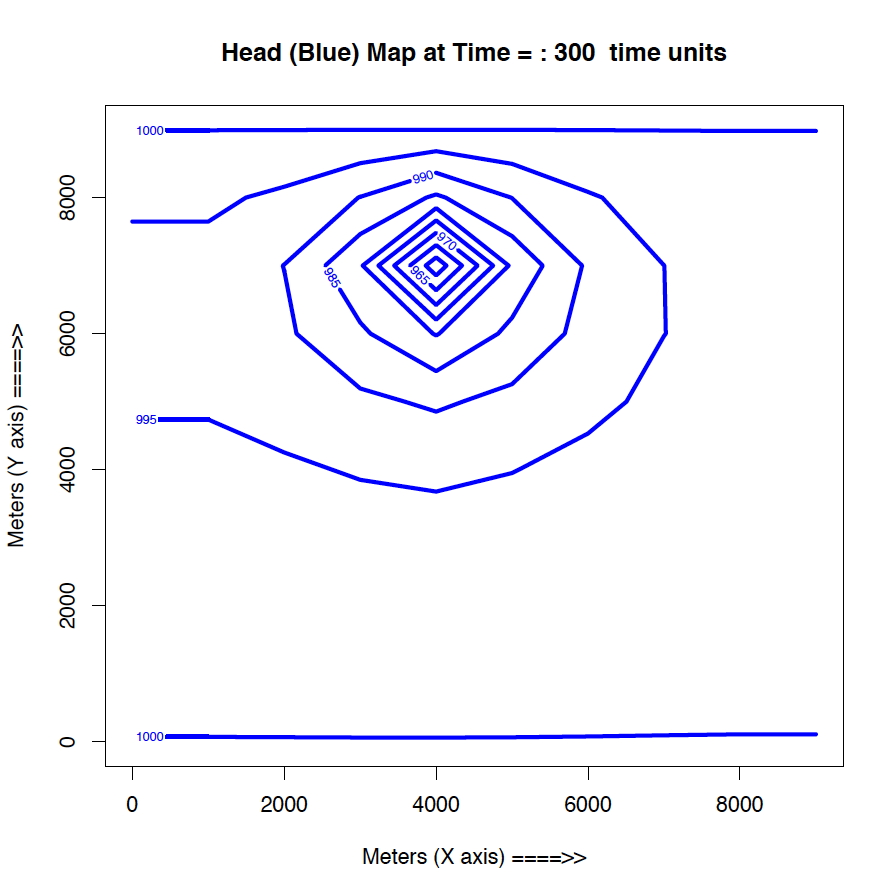
\includegraphics[height=4in]{./18-UnsteadyGroundwaterFlow/HubblevillePlot300.jpg} 
   \caption{Plot of head after 300 days of pumping}
   \label{fig:HubblevillePlot300}
\end{figure}

\begin{figure}[h!] %  figure placement: here, top, bottom, or page
   \centering
   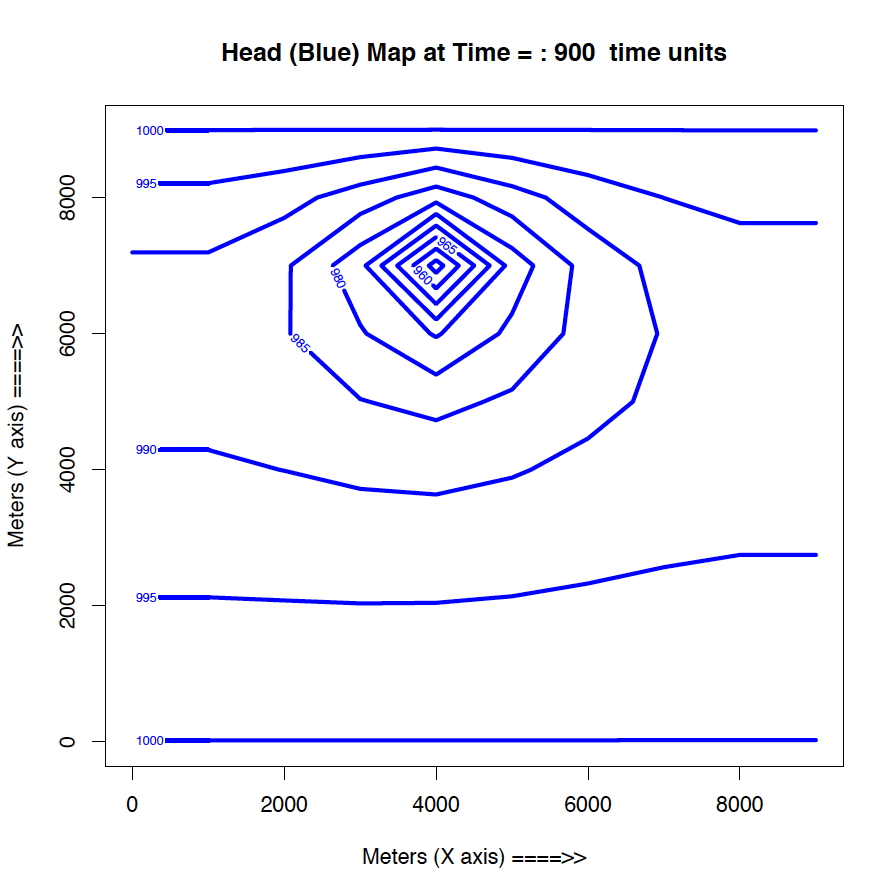
\includegraphics[height=4in]{./18-UnsteadyGroundwaterFlow/HubblevillePlot900.jpg} 
   \caption{Plot of head after 900 days of pumping}
   \label{fig:HubblevillePlot900}
\end{figure}


\clearpage

\subsection{Unconfined Aquifers}
As in the previous chapter, we will start with the unconfined flow equation in 2 dimensions

\begin{equation}
\begin{matrix}
S_{y} \Delta x \Delta y \frac{\partial h_i}{\partial t} = 
[ K_{x} \Delta y ~\overline{h}~ \frac{h_{i-1,j} - h_{i,j}}{\Delta x} +
 K_{y} \Delta x ~\overline{h}~ \frac{h_{i,j-1} - h_{i,j}}{\Delta y}] - \\
~~~~~~~~~~\\
~~~~~~~~~~[ K_{x} \Delta y ~\overline{h}~ \frac{h_{i,j} - h_{i+1,j}}{\Delta x} +
K_{y} \Delta x ~\overline{h}~ \frac{h_{i,j} - h_{i,j+1}}{\Delta y} ]        
\end{matrix}        
\end{equation}

Next divide by the cell plan view area $\Delta x \Delta y$ to obtain a more compact form of the difference equation.

\begin{equation}
\begin{matrix}
S \frac{\partial h_i}{\partial t} = 
[\frac{1}{\Delta x} K_{x}~\overline{h}~ \frac{h_{i-1,j} - h_{i,j}}{\Delta x} +
 \frac{1}{\Delta y} K_{y}~\overline{h}~ \frac{h_{i,j-1} - h_{i,j}}{\Delta y}] - \\
~~~~~~~~~~\\
~~~~~~~~~~[ \frac{1}{\Delta x} K_{x}~\overline{h}~  \frac{h_{i,j} - h_{i+1,j}}{\Delta x} +
  \frac{1}{\Delta y}  K_{y}~\overline{h}~ \frac{h_{i,j} - h_{i,j+1}}{\Delta y} ]        
\end{matrix}        
\end{equation}

Now finite-difference the left hand side and add pumping and recharge

\begin{equation}
\begin{matrix}
S \frac{h_i^{t+\Delta t}-h_i^{t}}{\Delta t} = 
[\frac{1}{\Delta x} K_{x}~\overline{h}~ \frac{h_{i-1,j} - h_{i,j}}{\Delta x} +
 \frac{1}{\Delta y} K_{y}~\overline{h}~ \frac{h_{i,j-1} - h_{i,j}}{\Delta y}] - \\
~~~~~~~~~~\\
~~~~~~~~~~[ \frac{1}{\Delta x} K_{x}~\overline{h}~  \frac{h_{i,j} - h_{i+1,j}}{\Delta x} +
  \frac{1}{\Delta y}  K_{y}~\overline{h}~ \frac{h_{i,j} - h_{i,j+1}}{\Delta y} ]          \\
  ~~~~~~~\\
  + \frac{R_{i,j}}{\Delta x \Delta y} - \frac{Q_{i,j}}{\Delta x \Delta y} \\     
\end{matrix}        
\end{equation}

Multiply through by $\Delta t$ and divide by $S_y$ (specific yield -- analogous to storage coefficient).

\begin{equation}
\begin{matrix}
h_i^{t+\Delta t}= h_i^{t} +
[\frac{\Delta t}{S_{y,i}~\Delta x} K_{x}~\overline{h}~ \frac{h_{i-1,j} - h_{i,j}}{\Delta x} +
 \frac{\Delta t}{S_{y,i}~\Delta y} K_{y}~\overline{h}~ \frac{h_{i,j-1} - h_{i,j}}{\Delta y}] - \\
~~~~~~~~~~\\
~~~~~~~~~~[ \frac{\Delta t}{S_{y,i}~\Delta x} K_{x}~\overline{h}~  \frac{h_{i,j} - h_{i+1,j}}{\Delta x} +
  \frac{\Delta t}{S_{y,i}~\Delta y}  K_{y}~\overline{h}~ \frac{h_{i,j} - h_{i,j+1}}{\Delta y} ]          \\
  ~~~~~~~\\
  + \frac{\Delta t~R_{i,j}}{S_{y,i}~\Delta x \Delta y} - \frac{\Delta t~Q_{i,j}}{S_{y,i}~\Delta x \Delta y} \\     
\end{matrix}        
\end{equation}

Next we will approximate the spatial variation of the $K~\overline{h}~$ as arithmetic mean values between two cells, so making the following definitions:

\begin{equation}
\begin{matrix}
A_{i,j} = \frac{\Delta t}{2 S_{y,i}~\Delta x^2}(K_{x,(i-1,j)} h_{i-1,j}+K_{x,(i,j)}h_{i,j}) \\ ~~ \\
B_{i,j} = \frac{\Delta t}{2 S_{y,i}~\Delta x^2}(K_{x,(i,j)}h_{i,j}+K_{x,(i+1,j)}h_{i+1,j})   \\ ~~ \\
C_{i,j} = \frac{\Delta t}{2 S_{y,i}~\Delta y^2}(K_{y,(i,j-1)}h_{i,j-1}+K_{y,(i,j)}h_{i,j})   \\ ~~ \\
D_{i,j} = \frac{\Delta t}{2 S_{y,i}~\Delta y^2}(K_{y,(i,j)}h_{i,j}+K_{y,(i,j+1)}h_{i,j+1})   \\ ~~ \\
E_{i,j} = \frac{\Delta t}{S_{y,i}~\Delta x \Delta y} 
\end{matrix}
\end{equation}

Collect the terms 

\begin{equation}
\begin{matrix}
h_i^{t+\Delta t} = h_i^{t} + \\
~~~~~~\\
~~~~~~   A_{i,j}h_{i-1,j}^{t^*} + B_{i,j}h_{i+1,j}^{t^*} - (A_{i,j}+B_{i,j}+C_{i,j}+D_{i,j})h_{i,j}^{t^*} + \\
~~~~~~\\
~~~~~~   C_{i,j}h_{i,j-1}^{t^*} + D_{i,j}h_{i,j+1}^{t^*} + E_{i,j}[R_{i,j}^{t^*}-Q_{i,j}^{t^*}]      \\
\end{matrix}        
\end{equation}

When we eventually decide whether to use explicit or implicit we will specify the time levels ($t^*$).   
As a practical matter the computation of the $A,B,C,D$ terms will have to be at a known or intermediate time level so it is not superscripted with a time level index -- although it is clear in the definition of the terms that a time level is needed to perform the requisite multiplications.

\subsubsection{Explicit Formulation}
The explicit formulation would specify the time levels on the right hand side as $t$.  
The resulting difference equation is
\begin{equation}
\begin{matrix}
h_i^{t+\Delta t} = h_i^{t} + \\
~~~~~~\\
~~~~~~   A_{i,j}h_{i-1,j}^{t} + B_{i,j}h_{i+1,j}^{t} - (A_{i,j}+B_{i,j}+C_{i,j}+D_{i,j})h_{i,j}^{t} + \\
~~~~~~\\
~~~~~~   C_{i,j}h_{i,j-1}^{t} + D_{i,j}h_{i,j+1}^{t} + E_{i,j}[R_{i,j}^{t}-Q_{i,j}^{t}]      \\
\end{matrix}        
\end{equation}

Everything on the right-hand side is known, so other than being conditionally stable (and using a small time step) we could start from known conditions and evolve the solution forward in time.  
There is non-linearity imbedded in the $A,B,C,D$ terms, but they are evaluated at known time levels.
As with the other unsteady case, the required time steps are small and dependent on the spatial and time step sizes, as well as the material properties. 
Unlike the previous case, the stability is also dependent on the solution itself and hence unpredictable in advance (although we can make very good guesses).

\subsubsection{Implicit Formulation}
The implicit formulation would specify the time levels on the right hand side as $t+ \Delta t$.
We would also have to decide how to handle the recharge and pumping -- either an average over two adjacent times, or at the old (or new) time level.
Here we choose the old time level, mostly for simplicity in building the \textbf{R} script.

The resulting difference equation is
\begin{equation}
\begin{matrix}
h_i^{t+\Delta t} = h_i^{t} + \\
~~~~~~\\
~~~~~~   A_{i,j}h_{i-1,j}^{t+ \Delta t} + B_{i,j}h_{i+1,j}^{t+ \Delta t} - (A_{i,j}+B_{i,j}+C_{i,j}+D_{i,j})h_{i,j}^{t+ \Delta t} + \\
~~~~~~\\
~~~~~~   C_{i,j}h_{i,j-1}^{t+ \Delta t} + D_{i,j}h_{i,j+1}^{t+ \Delta t} + E_{i,j}[R_{i,j}^{t}-Q_{i,j}^{t}]      \\
\end{matrix}        
\end{equation}

Observe that $h_i^{t+\Delta t}$ appears on both sides of the equation, so some additional manipulation is needed, first collect all the $h_i^{t+\Delta t}$ terms on the left side

\begin{equation}
\begin{matrix}
(A_{i,j}+B_{i,j}+C_{i,j}+D_{i,j}+1)h_i^{t+\Delta t} = h_i^{t} + \\
~~~~~~\\
~~~~~~   A_{i,j}h_{i-1,j}^{t+ \Delta t} + B_{i,j}h_{i+1,j}^{t+ \Delta t} + C_{i,j}h_{i,j-1}^{t+ \Delta t} + D_{i,j}h_{i,j+1}^{t+ \Delta t} + E_{i,j}[R_{i,j}^{t}-Q_{i,j}^{t}]      \\
\end{matrix}        
\end{equation}

Then divide both sides by the constant to get an update formula
\begin{equation}
h_i^{t+\Delta t} = 
\frac{h_i^{t} + A_{i,j}h_{i-1,j}^{t+ \Delta t} + B_{i,j}h_{i+1,j}^{t+ \Delta t} + C_{i,j}h_{i,j-1}^{t+ \Delta t} + D_{i,j}h_{i,j+1}^{t+ \Delta t} + E_{i,j}[R_{i,j}^{t}-Q_{i,j}^{t}] }{(A_{i,j}+B_{i,j}+C_{i,j}+D_{i,j}+1)} 
\end{equation}

The formula above is now structured so we can use our existing Jacobi iteration solver we developed in the previous chapter.
As we did for the steady case, we will simply move where the $A,B,C,D$ terms are computed.\footnote{They will go inside the Jacobi solver loop. We will pay a steep computational cost, but still be able to use our existing toolkit, handle the non-linearity by lagging the material properties a single iteration step, and still have an unconditionally stable solution method.}

Listing \ref{lst:2DUnsteadyUnconfined} is a listing that implements the revised finite-difference equation structure for the unconfined flow equation.
The new listing literally involved moving the portion of the steady, unconfined flow code that creates the variable transmissivity arrays to just before the assignment of boundary conditions in the unsteady confined code, and removing the existing instance of the unsteady confined code portion that created the $A,B,C,D$ portions.

The script was then tested (just to see if it runs) with the same Hubbleville input file.  
In the revised version, $\Delta z$ is still read into the program, but not actually used.  
Again this is an act of laziness as well as code re-usability.

\begin{lstlisting}[caption= Listing for \textbf{R} implementation for unsteady unconfined flow using Jacobi iteration , label=lst:2DUnsteadyUnconfined]
# 2D Unsteady Unconfined -- With Boundary Arrays and Wells
# 2D Aquifer Flow Model using Jacobi Iteration
# deallocate memory
rm(list=ls())
##############################################################
# prototype plotting function                                #
##############################################################
plotnow<-function(headnow,ncols,nrows,etime,deltat){
###    built position arrays for contour plotting         
velocity_plt<-matrix(0,ncols,nrows) 
for( i in 1:nrows){
  for( j in 1:ncols){
    velocity_plt[j,i]=headnow[i,j]
  }
}
###    contour plot of head -- note axes are rotated
#debug  message("elapsed time : ",maxtime * deltat)
mytitle <- paste("Head (Blue) Map at Time = :",etime*deltat," time units")
contour(distancex,distancey,velocity_plt,
        plot.title = title(main = mytitle,
                           xlab = "Meters (X axis) ====>>", 
                           ylab = "Meters (Y axis) ====>>"),
        col="blue",lwd=3,nlevels=10)
}
################################################################
################################################################
zz <- file("hubbleville.dat", "r") # Open a connection named zz to file named input.dat
# read the simulation conditons
deltax <-as.numeric(readLines(zz, n = 1, ok = TRUE, warn = TRUE,encoding = "unknown", skipNul = FALSE))
deltay <-as.numeric(readLines(zz, n = 1, ok = TRUE, warn = TRUE,encoding = "unknown", skipNul = FALSE))
deltaz <-as.numeric(readLines(zz, n = 1, ok = TRUE, warn = TRUE,encoding = "unknown", skipNul = FALSE))
deltat <-as.numeric(readLines(zz, n = 1, ok = TRUE, warn = TRUE,encoding = "unknown", skipNul = FALSE))
nrows <-as.numeric(readLines(zz, n = 1, ok = TRUE, warn = TRUE,encoding = "unknown", skipNul = FALSE))
ncols <-as.numeric(readLines(zz, n = 1, ok = TRUE, warn = TRUE,encoding = "unknown", skipNul = FALSE))
tolerance <- as.numeric(readLines(zz, n = 1, ok = TRUE, warn = TRUE,encoding = "unknown", skipNul = FALSE))
maxiter <- as.numeric(readLines(zz, n = 1, ok = TRUE, warn = TRUE,encoding = "unknown", skipNul = FALSE))
maxtime <- as.numeric(readLines(zz, n = 1, ok = TRUE, warn = TRUE,encoding = "unknown", skipNul = FALSE))
iprint <- as.numeric(readLines(zz, n = 1, ok = TRUE, warn = TRUE,encoding = "unknown", skipNul = FALSE))
distancex <- (readLines(zz, n = 1, ok = TRUE, warn = TRUE,encoding = "unknown", skipNul = FALSE))
distancey <- (readLines(zz, n = 1, ok = TRUE, warn = TRUE,encoding = "unknown", skipNul = FALSE))
# add boundary conditions 0= fixed head, 1= no flow
boundarytop <- (readLines(zz, n = 1, ok = TRUE, warn = TRUE,encoding = "unknown", skipNul = FALSE))
boundarybottom <- (readLines(zz, n = 1, ok = TRUE, warn = TRUE,encoding = "unknown", skipNul = FALSE))
boundaryleft <- (readLines(zz, n = 1, ok = TRUE, warn = TRUE,encoding = "unknown", skipNul = FALSE))
boundaryright <- (readLines(zz, n = 1, ok = TRUE, warn = TRUE,encoding = "unknown", skipNul = FALSE))
hydhead <-(readLines(zz, n = nrows, ok = TRUE, warn = TRUE,encoding = "unknown", skipNul = FALSE))
# hydhead is now the initial condition array #
hydcondx <-(readLines(zz, n = nrows, ok = TRUE, warn = TRUE,encoding = "unknown", skipNul = FALSE))
hydcondy <-(readLines(zz, n = nrows, ok = TRUE, warn = TRUE,encoding = "unknown", skipNul = FALSE))
storage <-(readLines(zz, n = nrows, ok = TRUE, warn = TRUE,encoding = "unknown", skipNul = FALSE))
pumping <-(readLines(zz, n = nrows, ok = TRUE, warn = TRUE,encoding = "unknown", skipNul = FALSE)) 
close(zz)
# split the multiple column strings into numeric components for a vector
distancex <-as.numeric(unlist(strsplit(distancex,split=" ")))
distancey <-as.numeric(unlist(strsplit(distancey,split=" ")))
boundarytop <-as.numeric(unlist(strsplit(boundarytop,split=" ")))
boundarybottom <-as.numeric(unlist(strsplit(boundarybottom,split=" ")))
boundaryleft <-as.numeric(unlist(strsplit(boundaryleft,split=" ")))
boundaryright <-as.numeric(unlist(strsplit(boundaryright,split=" ")))
hydhead <-as.numeric(unlist(strsplit(hydhead,split=" ")))
hydcondx <-as.numeric(unlist(strsplit(hydcondx,split=" ")))
hydcondy <-as.numeric(unlist(strsplit(hydcondy,split=" ")))
storage <-as.numeric(unlist(strsplit(storage,split=" ")))
pumping <-as.numeric(unlist(strsplit(pumping,split=" ")))
# convert the numeric vectors into matrices for easier indexing
hydhead <- matrix(hydhead,nrow=nrows,ncol=ncols,byrow = TRUE)
hydcondx <-matrix(hydcondx,nrow=nrows,ncol=ncols,byrow = TRUE)
hydcondy <-matrix(hydcondy,nrow=nrows,ncol=ncols,byrow = TRUE)
storage <-matrix(storage,nrow=nrows,ncol=ncols,byrow = TRUE)
pumping <-matrix(pumping,nrow=nrows,ncol=ncols,byrow = TRUE)
# allocate a graphics device for sequential plotting
pdf("2d-unsteady-confined-junk.plot.pdf") # send any plots to file
# here we perform the velocity potential calculations
# built the transmissivity arrays
amat<-matrix(0,nrows,ncols) 
bmat<-matrix(0,nrows,ncols) 
cmat<-matrix(0,nrows,ncols)
dmat<-matrix(0,nrows,ncols)
qrat<-matrix(0,nrows,ncols)
for(irow in 2:(nrows-1)){
  for(jcol in 2:(ncols-1)){
      #    amat[irow,jcol]<-((hydcondx[irow-1,jcol  ]+hydcondx[irow  ,jcol  ])*deltat*deltaz)/(2.0*storage[irow,jcol]*deltax^2)
    #    bmat[irow,jcol]<-((hydcondx[irow  ,jcol  ]+hydcondx[irow+1,jcol  ])*deltat*deltaz)/(2.0*storage[irow,jcol]*deltax^2)
    #    cmat[irow,jcol]<-((hydcondy[irow  ,jcol-1]+hydcondy[irow  ,jcol  ])*deltat*deltaz)/(2.0*storage[irow,jcol]*deltay^2)
    #    dmat[irow,jcol]<-((hydcondy[irow  ,jcol  ]+hydcondy[irow  ,jcol+1])*deltat*deltaz)/(2.0*storage[irow,jcol]*deltay^2)
    qrat[irow,jcol]<-(-1.0)*deltat*pumping[irow,jcol]/(deltax*deltay*storage[irow,jcol])
    }
}
# for(irow in 2:(nrows-1)){
#   for(jcol in 2:(ncols-1)){
#     amat[irow,jcol]<-((hydcondx[irow-1,jcol  ]+hydcondx[irow  ,jcol  ])*deltaz)/(2.0*deltax^2)
#     bmat[irow,jcol]<-((hydcondx[irow  ,jcol  ]+hydcondx[irow+1,jcol  ])*deltaz)/(2.0*deltax^2)
#     cmat[irow,jcol]<-((hydcondy[irow  ,jcol-1]+hydcondy[irow  ,jcol  ])*deltaz)/(2.0*deltay^2)
#     dmat[irow,jcol]<-((hydcondy[irow  ,jcol  ]+hydcondy[irow  ,jcol+1])*deltaz)/(2.0*deltay^2)
#   }
# }
####### initial conditions ######################################
print(hydhead)
#maxtime <- 1
headnow <- hydhead
for (tstep in 1:maxtime){
###### use jacobi to solve for a single time step ###############
hydhead <- headnow
headold <- hydhead # copy the head array, used to test for stopping
tolflag <- FALSE
for (iter in 1:maxiter){
# built the variable transmissivity arrays for current time-step
    for(irow in 2:(nrows-1)){
        for(jcol in 2:(ncols-1)){
            amat[irow,jcol]<-((hydcondx[irow-1,jcol  ]*hydhead[irow-1,jcol  ]
            +hydcondx[irow  ,jcol  ]*hydhead[irow  ,jcol  ]))/(2.0*deltax^2)
            
            bmat[irow,jcol]<-((hydcondx[irow  ,jcol  ]*hydhead[irow  ,jcol  ]
            +hydcondx[irow+1,jcol  ]*hydhead[irow+1,jcol  ]))/(2.0*deltax^2)
            
            cmat[irow,jcol]<-((hydcondy[irow  ,jcol-1]*hydhead[irow  ,jcol-1]
            +hydcondy[irow  ,jcol  ]*hydhead[irow  ,jcol  ]))/(2.0*deltay^2)
            
            dmat[irow,jcol]<-((hydcondy[irow  ,jcol  ]*hydhead[irow  ,jcol  ]
            +hydcondy[irow  ,jcol+1]*hydhead[irow  ,jcol+1]))/(2.0*deltay^2)
            
        }
    }
# set the boundary conditions
for(jcol in 1:ncols){ #top and bottom rows
    if(boundarytop[jcol] == 0){hydhead[1,jcol]<-hydhead[2,jcol]} #no-flow at top
    if(boundarybottom[jcol] == 0){hydhead[nrows,jcol]<-hydhead[2,jcol]} #no-flow at bottom
    # otherwise values are fixed head
}
for(irow in 1:nrows){  #left and right columns
    if(boundaryleft[irow] == 0){hydhead[irow,1]<-hydhead[irow,2]} #no-flow at left
    if(boundaryright[irow] == 0){hydhead[irow,ncols]<-hydhead[irow,ncols-1]} #no-flow at right
    # otherwise values are fixed head
}
  for (irow in 2:(nrows-1)){
    for (jcol in 2:(ncols-1)){
      hydhead[irow,jcol] <- (  headnow[irow,jcol] +
                                  qrat[irow,jcol] +
           amat[irow,jcol]*hydhead[irow-1,jcol  ] +
           bmat[irow,jcol]*hydhead[irow+1,jcol  ] +
           cmat[irow,jcol]*hydhead[irow  ,jcol-1] +
           dmat[irow,jcol]*hydhead[irow  ,jcol+1] )/
        (amat[irow,jcol]+bmat[irow,jcol]+cmat[irow,jcol]+dmat[irow,jcol]+1)
    }
  }
  # test for stopping iterations
  percentdiff <- sum((hydhead-headold)^2)
  if (percentdiff < tolerance){
    message("Exit iterations in velocity potential because tolerance met");
    message("Iterations =", iter);
    message("Current error : ",percentdiff);
    tolflag <- TRUE
    break
  }
 headold<-hydhead  #update the current head vector
# if( iter %% 1000 == 0){message("Calculating in Potential Function ",iter," of ",maxiter, " iterations")}
}
if (tolflag == FALSE){
#  message("Exit iterations in potential function at max iterations")
  message("Current error : ",percentdiff)
  }
# perform an update
headnow <- hydhead
########## end of a time step ################################
#print(headnow)
# check for plotnow
if(tstep%%iprint==0){plotnow(headnow,ncols,nrows,tstep,deltat)}
}
# output ending conditons
write(t(hydhead), file='2d-unsteady-confined.txt',ncolumns = ncols,sep=",")
# deallocate (disconnect) graphics device
dev.off() # disconect the pdf file
\end{lstlisting}

\textbf{Example 2: Unconfined Rectangular Aquifer with Pumping -- Unsteady Flow}\\
Figure \ref{fig:Hubbleville2} is a plan view of an unconfined aquifer with a Well field located as shown, near the Red River.
The head in the river is 1000 meters as is the head at the South boundary, the Green Swamp.
The well field pumps 20,000 cubic meters per day.
The net recharge to the aquifer is 0.001 meters/day.
The hydraulic conductivity of the aquifer is 50 meters per day.
The hydraulic conductivity of the swamp is about 500 meters per day.
The specific yield of the aquifer is 0.35.
The town of Hubbleville is at elevation 1020 meters.
The managers of the Green Swamp Conservation area are concerned that pumping will significantly reduce groundwater
discharge to the swamp and threaten wildlife habitat. 
The town claims that the well is located sufficiently close to the Red River so that induced recharge will contribute the significant portion of water that flows to the well and none will come from the swamp.
Each cell in the sketch is $1000 X 1000$ meters.

Use the unsteady, unconfined groundwater flow script to
\begin{enumerate}
\item Demonstrate that flow is towards the swamp with the well field inactive (zero pumping, but non-zero recharge).
\item Determine if the flow is still towards the swamp with the well field activated (non-zero pumping, non-zero recharge).
\item Assuming that water is eventually drawn from the swamp, determine how many years the well field can be operated, before water is drawn from the swamp into the well, or until the well de-waters (head drops below zero).
\end{enumerate}

\begin{figure}[h!] %  figure placement: here, top, bottom, or page
   \centering
   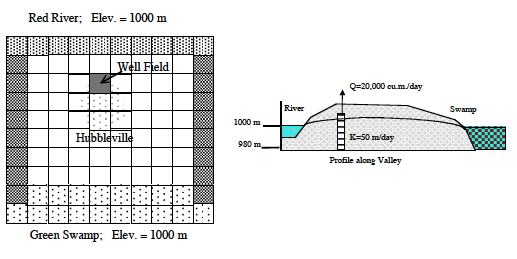
\includegraphics[width=6in]{./18-UnsteadyGroundwaterFlow/Hubbleville2.jpg} 
   \caption{Hubbleville Aquifer System}
   \label{fig:Hubbleville3}
\end{figure}

Answering these three questions is a matter of running our script three times, with two input files. 
The first input file would be the problem conditions with the well off, but with recharge on.
Given that our prototype script does not have a recharge array, we have two choices --- add one and refactor the requesite parts of the script, or observe that recharge is just negative pumping and simply change the pumping array.  
I chose that second approach, the first is left as an exercise.
So the recharge for any cell in the correct problem units is 
\begin{equation}
R_{i,j} = rate \times \Delta x \times \Delta y = 0.001~m/day~\times 1000~m~\times 1000~m = 1000 m^3/day
\end{equation}

The first question is asking about a ``pre-development'' condition, so we need to run our script once until the solution stops changing (an equilibrium solution) then use the head distribution for this solution as the initial condition for the second run, when we turn on the pump.
An important observation is that the aquifer bottom elevation is at 980 meters, so the hydraulic head in the swamp or at the river is only 20 meters based on the profile sketch.
Thus the maximum head in the aquifer should be less than 1020 meters (otherwise the whole area is a swamp) and greater that zero.
Once the computations are completed we can add back the datum (980 meters) to recover the various water elevations if we wish.
For the example, I will just stipulate the desired head is between zero and 40 meters.

Listing \ref{lst:Hubbleville2} is the input file for the pre-development conditions. 
The file was created by running the script once with all the heads set to 20.  
Then at the end of the run (30 years), the output heads were pasted back into the input file, and it was rerun.
This process was repeated several times until the program ran through all the time steps using only a single iteration and the error term essentially reported as a small constant value.
At this condition, the system was deemed to be at equilibrium.  
The listing shows the result that was used to produce Figure \ref{fig:HubblevillePlot30PreDev}.

Examination of Figure \ref{fig:HubblevillePlot30PreDev} shows that the contour lines are parallel to the swamp and the river (bottom and top) and slope from the middle (Y == 5500 meters) towards each boundary. 
The highest plotted water elevation is 34 meters, which would be a depth of about 6 meters beneath the town of Hubbleville.
The high ``ridge'' is called a groundwater divide.  
All water South of the divide flows to the swamp, whereas all water North of the divide flows to the river.

\begin{lstlisting}[caption= Input file for the Hubleville probelm -- but as an unconfined aquifer -- model is run to equilibrium to establish the pre-development conditions.  Here we choose to use 30 years simulation time as sufficiently long and printed contour maps at 5 year intervals to assess if there is much change as the solution proceeds , label=lst:Hubbleville2]
1000
1000
10
1
10
10
1e-8
1000
10950
1825
0 1000 2000 3000 4000 5000 6000 7000 8000 9000 
0 1000 2000 3000 4000 5000 6000 7000 8000 9000
1 1 1 1 1 1 1 1 1 1 
1 1 1 1 1 1 1 1 1 1
0 0 0 0 0 0 0 0 0 0
0 0 0 0 0 0 0 0 0 0
20 20 20 20 20 20 20 20 20 20
21.33491 21.33491 21.33491 21.33491 21.33491 21.33491 21.33491 21.33491 21.33491 21.33491
23.18453 23.18453 23.18453 23.18453 23.18453 23.18453 23.18453 23.18453 23.18453 23.18453
29.33826 29.33826 29.33826 29.33826 29.33826 29.33826 29.33826 29.33826 29.33826 29.33826
32.70564 32.70564 32.70564 32.70564 32.70564 32.70564 32.70564 32.70564 32.70564 32.70564
34.12182 34.12182 34.12182 34.12182 34.12182 34.12182 34.12182 34.12182 34.12182 34.12182
33.83271 33.83271 33.83271 33.83271 33.83271 33.83271 33.83271 33.83271 33.83271 33.83271
31.79183 31.79183 31.79183 31.79183 31.79183 31.79183 31.79183 31.79183 31.79183 31.79183
27.61346 27.61346 27.61346 27.61346 27.61346 27.61346 27.61346 27.61346 27.61346 27.61346
20 20 20 20 20 20 20 20 20 20
500 500 500 500 500 500 500 500 500 500
500 500 500 500 500 500 500 500 500 500
50 50 50 50 50 50 50 50 50 50
50 50 50 50 50 50 50 50 50 50
50 50 50 50 50 50 50 50 50 50
50 50 50 50 50 50 50 50 50 50
50 50 50 50 50 50 50 50 50 50
50 50 50 50 50 50 50 50 50 50
50 50 50 50 50 50 50 50 50 50
50 50 50 50 50 50 50 50 50 50
500 500 500 500 500 500 500 500 500 500
500 500 500 500 500 500 500 500 500 500
50 50 50 50 50 50 50 50 50 50
50 50 50 50 50 50 50 50 50 50
50 50 50 50 50 50 50 50 50 50
50 50 50 50 50 50 50 50 50 50
50 50 50 50 50 50 50 50 50 50
50 50 50 50 50 50 50 50 50 50
50 50 50 50 50 50 50 50 50 50
50 50 50 50 50 50 50 50 50 50
0.35 0.35 0.35 0.35 0.35 0.35 0.35 0.35 0.35 0.35
0.35 0.35 0.35 0.35 0.35 0.35 0.35 0.35 0.35 0.35
0.35 0.35 0.35 0.35 0.35 0.35 0.35 0.35 0.35 0.35
0.35 0.35 0.35 0.35 0.35 0.35 0.35 0.35 0.35 0.35
0.35 0.35 0.35 0.35 0.35 0.35 0.35 0.35 0.35 0.35
0.35 0.35 0.35 0.35 0.35 0.35 0.35 0.35 0.35 0.35
0.35 0.35 0.35 0.35 0.35 0.35 0.35 0.35 0.35 0.35
0.35 0.35 0.35 0.35 0.35 0.35 0.35 0.35 0.35 0.35
0.35 0.35 0.35 0.35 0.35 0.35 0.35 0.35 0.35 0.35
0.35 0.35 0.35 0.35 0.35 0.35 0.35 0.35 0.35 0.35
-1000 -1000 -1000 -1000 -1000 -1000 -1000 -1000 -1000 -1000
-1000 -1000 -1000 -1000 -1000 -1000 -1000 -1000 -1000 -1000
-1000 -1000 -1000 -1000 -1000 -1000 -1000 -1000 -1000 -1000
-1000 -1000 -1000 -1000 -1000 -1000 -1000 -1000 -1000 -1000
-1000 -1000 -1000 -1000 -1000 -1000 -1000 -1000 -1000 -1000
-1000 -1000 -1000 -1000 -1000 -1000 -1000 -1000 -1000 -1000
-1000 -1000 -1000 -1000 -1000 -1000 -1000 -1000 -1000 -1000
-1000 -1000 -1000 -1000 -1000 -1000 -1000 -1000 -1000 -1000
-1000 -1000 -1000 -1000 -1000 -1000 -1000 -1000 -1000 -1000
-1000 -1000 -1000 -1000 -1000 -1000 -1000 -1000 -1000 -1000
\end{lstlisting}

\begin{figure}[h!] %  figure placement: here, top, bottom, or page
   \centering
   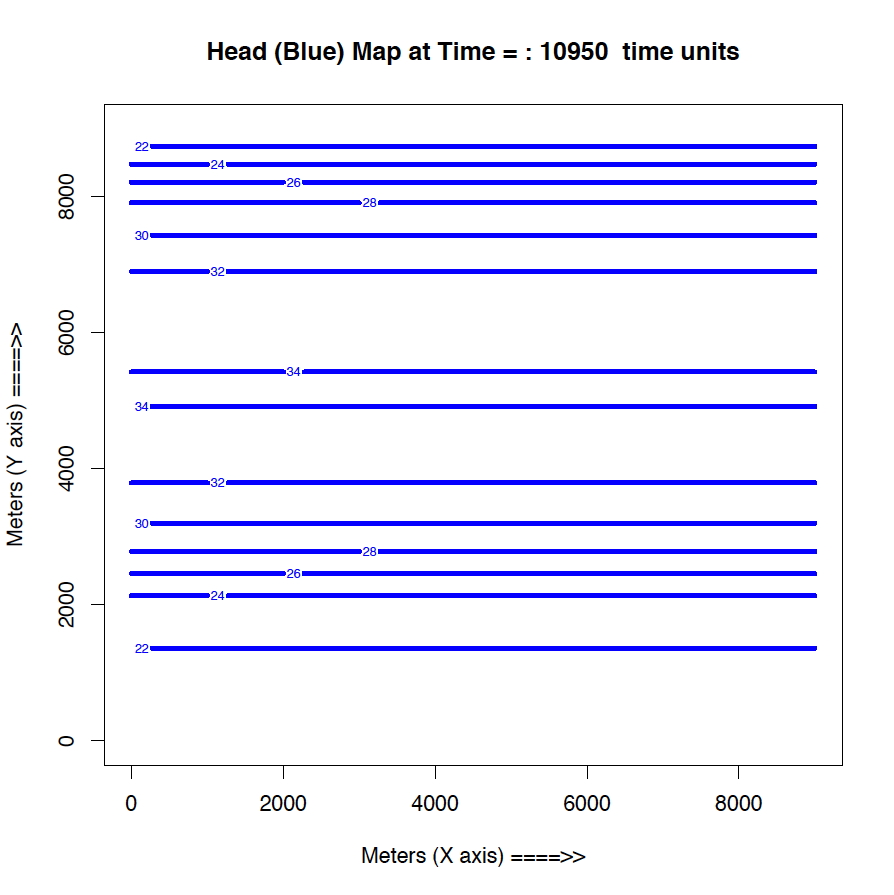
\includegraphics[width=6in]{./18-UnsteadyGroundwaterFlow/HubblevillePlot30PreDev.jpg} 
   \caption{Hubbleville Aquifer head distribution at equilibrium}
   \label{fig:HubblevillePlot30PreDev}
\end{figure}

Now we will activate the pumping.  
The pumping rate is positive 20,000 cubic meters per day.  
The recharge rate is a negative 1,000 cubic meters per day, so net pumping is 19,000 cubic meters per day.
We will change the contents of the single well field cell, rename the file, and rerun the script.

Figure \ref{fig:HubblevillePlot5PostDev} is the result of the change.
The plot is promising because the slope of the water is still towards the swamp.
However, if we examine the plot at 30 years we will discover we have dewatered the aquifer in the wellfield (at some point the wells would fail).
So we can conclude that the swamp is safe, but the town of Hubbleville cannot realistically recover the amount of water they desire.

While we have the model available, we can try different pumping rates to see how much firm yield the town could expect.
For the example, lets stipulate that the smallest allowable head in the well field is 5 meters.
Our goal is now to determine how large a pumping rate we can use and keep the head at this location greater than 5 meters.
The exercise is quite simple, we will change the pumping value and run the script and examine the output.  
If the head is too small, decrease the pumping, if the head is too large then increase the pumping and we stop when it is just right.\footnote{Goldilocks optimization!}

\begin{figure}[h!] %  figure placement: here, top, bottom, or page
   \centering
   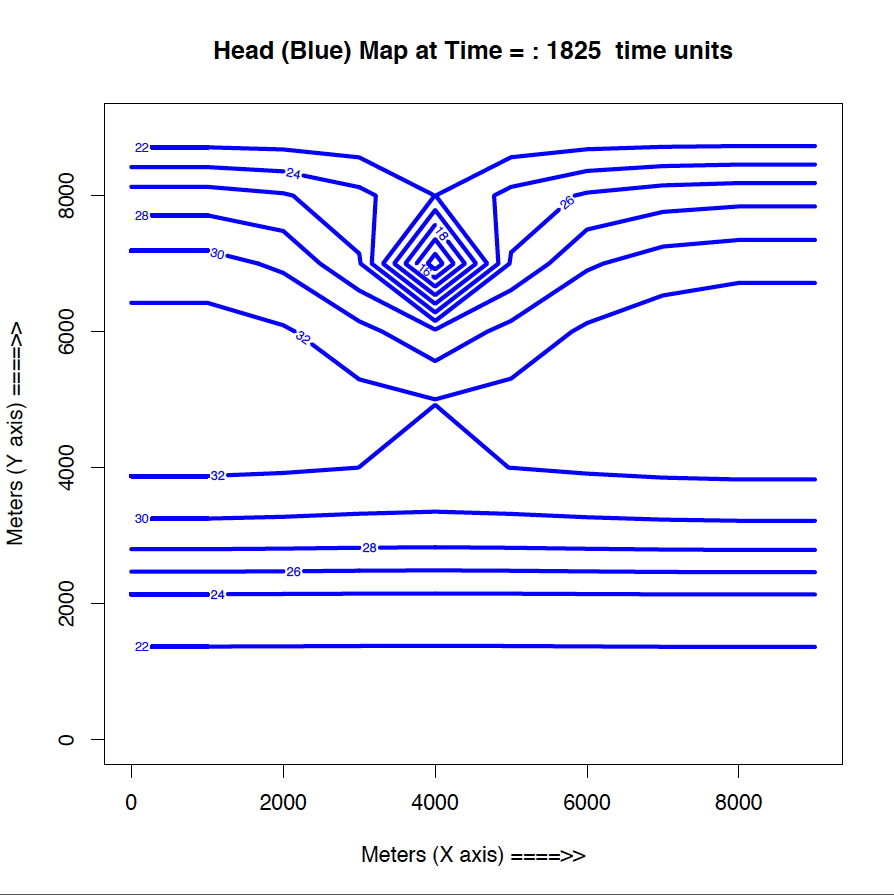
\includegraphics[width=6in]{./18-UnsteadyGroundwaterFlow/HubblevillePlot5PostDev.jpg} 
   \caption{Hubbleville Aquifer head distribution at 5 years after well field is active}
   \label{fig:HubblevillePlot5PostDev}
\end{figure}

Listing \ref{lst:Hubbleville3} is the input file used for the post development case with a pumping rate set to 18,000 cubic meters per day.
The simulation forecast that the head in the well field cell would be 6.55 meters after 60 years of pumping.  
The stopping criteria for each time step was still changing, hence we have not quite reached equilibrium -- however it would be safe to conclude that a firm yield of 18,000 cubic meters per day is achievable and does not impact the swamp as was feared in the original problem statement.

Figure \ref{fig:HubblevillePlot60PostDev} is the contour plot of the head distribution under these conditions.
The induced recharge from the river is evident by the contour that extends to the boundary at the top.
The swamp is South of the saddle point in the water table plot and water south of this point flows towards the swamp (as desired).
\begin{lstlisting}[caption= Input file for the Hubleville probelm -- 60 year simulation.  Pumping rate is 18000 cubic meters per day , label=lst:Hubbleville3]
1000
1000
10
1
10
10
1e-8
1000
21900
2190
0 1000 2000 3000 4000 5000 6000 7000 8000 9000 
0 1000 2000 3000 4000 5000 6000 7000 8000 9000
1 1 1 1 1 1 1 1 1 1 
1 1 1 1 1 1 1 1 1 1
0 0 0 0 0 0 0 0 0 0
0 0 0 0 0 0 0 0 0 0
20 20 20 20 20 20 20 20 20 20
21.33491 21.33491 21.33491 21.33491 21.33491 21.33491 21.33491 21.33491 21.33491 21.33491
23.18453 23.18453 23.18453 23.18453 23.18453 23.18453 23.18453 23.18453 23.18453 23.18453
29.33826 29.33826 29.33826 29.33826 29.33826 29.33826 29.33826 29.33826 29.33826 29.33826
32.70564 32.70564 32.70564 32.70564 32.70564 32.70564 32.70564 32.70564 32.70564 32.70564
34.12182 34.12182 34.12182 34.12182 34.12182 34.12182 34.12182 34.12182 34.12182 34.12182
33.83271 33.83271 33.83271 33.83271 33.83271 33.83271 33.83271 33.83271 33.83271 33.83271
31.79183 31.79183 31.79183 31.79183 31.79183 31.79183 31.79183 31.79183 31.79183 31.79183
27.61346 27.61346 27.61346 27.61346 27.61346 27.61346 27.61346 27.61346 27.61346 27.61346
20 20 20 20 20 20 20 20 20 20
500 500 500 500 500 500 500 500 500 500
500 500 500 500 500 500 500 500 500 500
50 50 50 50 50 50 50 50 50 50
50 50 50 50 50 50 50 50 50 50
50 50 50 50 50 50 50 50 50 50
50 50 50 50 50 50 50 50 50 50
50 50 50 50 50 50 50 50 50 50
50 50 50 50 50 50 50 50 50 50
50 50 50 50 50 50 50 50 50 50
50 50 50 50 50 50 50 50 50 50
500 500 500 500 500 500 500 500 500 500
500 500 500 500 500 500 500 500 500 500
50 50 50 50 50 50 50 50 50 50
50 50 50 50 50 50 50 50 50 50
50 50 50 50 50 50 50 50 50 50
50 50 50 50 50 50 50 50 50 50
50 50 50 50 50 50 50 50 50 50
50 50 50 50 50 50 50 50 50 50
50 50 50 50 50 50 50 50 50 50
50 50 50 50 50 50 50 50 50 50
0.35 0.35 0.35 0.35 0.35 0.35 0.35 0.35 0.35 0.35
0.35 0.35 0.35 0.35 0.35 0.35 0.35 0.35 0.35 0.35
0.35 0.35 0.35 0.35 0.35 0.35 0.35 0.35 0.35 0.35
0.35 0.35 0.35 0.35 0.35 0.35 0.35 0.35 0.35 0.35
0.35 0.35 0.35 0.35 0.35 0.35 0.35 0.35 0.35 0.35
0.35 0.35 0.35 0.35 0.35 0.35 0.35 0.35 0.35 0.35
0.35 0.35 0.35 0.35 0.35 0.35 0.35 0.35 0.35 0.35
0.35 0.35 0.35 0.35 0.35 0.35 0.35 0.35 0.35 0.35
0.35 0.35 0.35 0.35 0.35 0.35 0.35 0.35 0.35 0.35
0.35 0.35 0.35 0.35 0.35 0.35 0.35 0.35 0.35 0.35
-1000 -1000 -1000 -1000 -1000 -1000 -1000 -1000 -1000 -1000
-1000 -1000 -1000 -1000 -1000 -1000 -1000 -1000 -1000 -1000
-1000 -1000 -1000 -1000 -1000 -1000 -1000 -1000 -1000 -1000
-1000 -1000 -1000 -1000 -1000 -1000 -1000 -1000 -1000 -1000
-1000 -1000 -1000 -1000 -1000 -1000 -1000 -1000 -1000 -1000
-1000 -1000 -1000 -1000 -1000 -1000 -1000 -1000 -1000 -1000
-1000 -1000 -1000 -1000 -1000 -1000 -1000 -1000 -1000 -1000
-1000 -1000 -1000 -1000 17000 -1000 -1000 -1000 -1000 -1000
-1000 -1000 -1000 -1000 -1000 -1000 -1000 -1000 -1000 -1000
-1000 -1000 -1000 -1000 -1000 -1000 -1000 -1000 -1000 -1000
\end{lstlisting}


\begin{figure}[h!] %  figure placement: here, top, bottom, or page
   \centering
   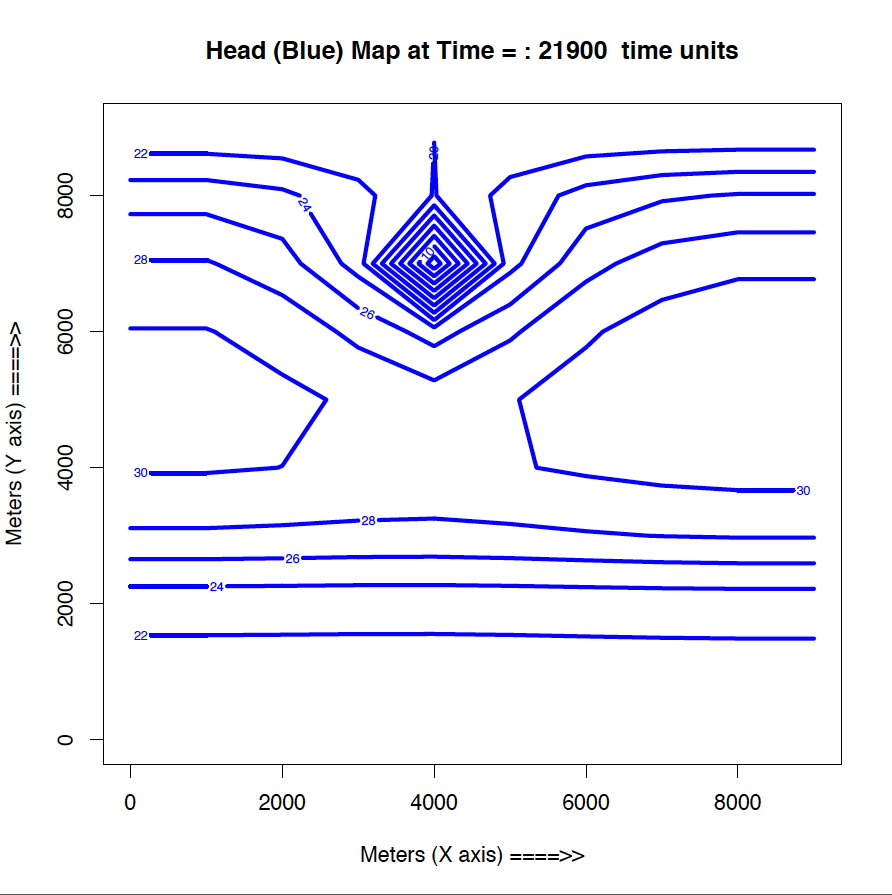
\includegraphics[width=6in]{./18-UnsteadyGroundwaterFlow/HubblevillePlot60PostDev.jpg} 
   \caption{Hubbleville Aquifer head distribution at 60 years after well field is active with pumping rate of 18,000 meters per day}
   \label{fig:HubblevillePlot60PostDev}
\end{figure}

These three chapters introduced an important computational hydraulics problem -- namely that of flow in a porous medium. 
The governing equation of motion is Darcy's law.  
We computed the heads using a variety of methods, but mostly focused on Jacobi iteration because for these kinds of problems it is a stable solution technique.  
It is not particularly computationally efficient, but it works. 

We choose not to even do explicit methods -- not because they are bad, but because they are conditionally stable which can be an undesired problem.  
\footnote{Explicit methods are easy to program, and if I were tasked with simulating an explosion (a chemical reaction that moves outward from ignition at or above the speed of sound) or some other process that is not well documented, I would start with an explicit approach because I could get code up and running quickly and identify other problems that might be encountered along the way.}
We also focused on code reuse so the reader can look back over the three chapters and see the evolution of the code as the problem got more complex.

Lastly, while not apparent, we have replicated much of the internal functionality of the professional code \texttt{MODFLOW} which we could compare our work to if we had to use the \textbf{R} script for something the professional code does not do easily. 
The scripts here are very crude -- to professionalize them we would want to add the concept of ``layers'' so we could do 3D models, and want to generalize the file reading components of the tool.  
We would also want to move much of the computation engine components into their own prototype functions so the structure of the program is easier to understand and maintain.
Nevertheless, if you have worked this far, you have seen what's under the hood of a groundwater flow code.\footnote{Actually you have also seen the code one would use for linear heat flow computations -- because the PDEs look the same, hence the solvers will work the same.}


\subsection{Exercises}
\begin{enumerate}
\item Figure \ref{fig:ES1-1} is a plan view of a confined aquifer system bounded by mountains (no-flow) and a river (constant head).
The 10 meter thick aquifer is approximately horizontal. 
The material properties are reported as transmissivities ($T = K \times$thickness).
The storage coefficient for the aquifer system is 0.05.
\begin{figure}[h!] %  figure placement: here, top, bottom, or page
   \centering
   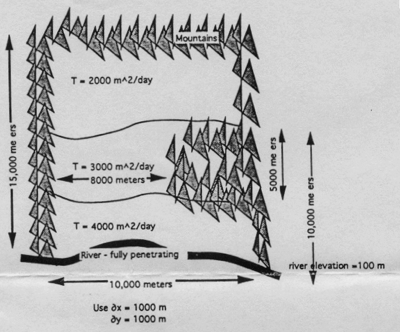
\includegraphics[width=5in]{./18-UnsteadyGroundwaterFlow/EX1-1.jpg} 
   \caption{Aquifer system bounded on three sides with mountains, and one side by a river.  The aquifer is about 10 meters thick at the river}
   \label{fig:ES1-1}
\end{figure}
Figure \ref{fig:ES1-2} is the same aquifer system with a recharge gallery and a well field. 
\begin{figure}[h!] %  figure placement: here, top, bottom, or page
   \centering
   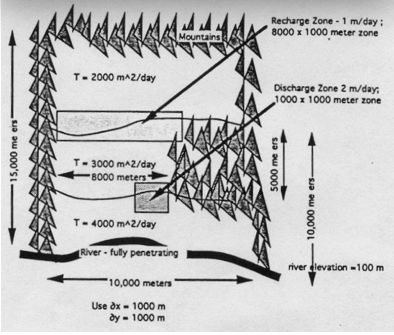
\includegraphics[width=5in]{./18-UnsteadyGroundwaterFlow/EX1-2.jpg} 
   \caption{Aquifer system bounded on three sides with mountains, and one side by a river.  The aquifer is about 10 meters thick at the river.  A recharge gallery is shown where water in recharged into the aquifer.  A discharge gallery (wellfield) is shown where water is removed from the aquifer.}
   \label{fig:ES1-2}
\end{figure}
\begin{enumerate}
\item Develop or modify an  \textbf{R} script to simulate the unsteady confined aquifer system shown.  
Build your tool so that recharge and pumping are read in as separate arrays.
To handle the mountain intrusion into the plain from the East in the sketch you will either have to modify how your script implements boundary conditions, or treat the mountain range as a low-permeability (small $T$) inclusion into the aquifer.
\item Run your script and produce a contour plot of the head distribution in the pre-development case at equilibrium.
\item Describe how you decided equilibrium is reached.
\item Compare your equilibrium solution to the same problem conditions run using your steady-flow solver.  
\item Run the script with the post-development case, and produce contour plots of the head distribution at 5 and 10 years of operation.
\item Estimate the fraction of recharge water that is captured by the well field, assuming the 10-year contour plot is an equilibrium condition.
\end{enumerate}

\item Repeat Example 2 with the following changes:
\begin{enumerate}
\item Modify the script (or build your own) that reads recharge as a separate array (instead of the R-P hack that was employed in the example).
\item Assume cloud seeding doubles the average recharge rate.  Determine the amount of water that can be pumped from the well field such that the head in the wellfield is greater than 5 meters after 60 years of pumping.
\item Produce a contour map of the head distribution at your solution.
\end{enumerate}

\item (Advanced) Modify your scripts to allow for different stress periods -- intervals of time where recharge and pumping remain constant but where different stress periods can have different recharge and pumping rates.  Develop examples to illustrate the effect of the modification.
\item (Advanced) Modify the scripts to multiple layers to approximate a 3D aquifer system.   You will need to modify the difference equations to simulate the vertical flow component between the layers.
\end{enumerate}
